\documentclass[11pt,]{article}
\usepackage{lmodern}
\usepackage{amssymb,amsmath}
\usepackage{ifxetex,ifluatex}
\usepackage{fixltx2e} % provides \textsubscript
\ifnum 0\ifxetex 1\fi\ifluatex 1\fi=0 % if pdftex
  \usepackage[T1]{fontenc}
  \usepackage[utf8]{inputenc}
\else % if luatex or xelatex
  \ifxetex
    \usepackage{mathspec}
  \else
    \usepackage{fontspec}
  \fi
  \defaultfontfeatures{Ligatures=TeX,Scale=MatchLowercase}
\fi
% use upquote if available, for straight quotes in verbatim environments
\IfFileExists{upquote.sty}{\usepackage{upquote}}{}
% use microtype if available
\IfFileExists{microtype.sty}{%
\usepackage{microtype}
\UseMicrotypeSet[protrusion]{basicmath} % disable protrusion for tt fonts
}{}
\usepackage[margin=1in]{geometry}
\usepackage{hyperref}
\hypersetup{unicode=true,
            pdftitle={Ruby Plotting with Galaaz},
            pdfauthor={Rodrigo Botafogo},
            pdfborder={0 0 0},
            breaklinks=true}
\urlstyle{same}  % don't use monospace font for urls
\usepackage{color}
\usepackage{fancyvrb}
\newcommand{\VerbBar}{|}
\newcommand{\VERB}{\Verb[commandchars=\\\{\}]}
\DefineVerbatimEnvironment{Highlighting}{Verbatim}{commandchars=\\\{\}}
% Add ',fontsize=\small' for more characters per line
\usepackage{framed}
\definecolor{shadecolor}{RGB}{248,248,248}
\newenvironment{Shaded}{\begin{snugshade}}{\end{snugshade}}
\newcommand{\AlertTok}[1]{\textcolor[rgb]{0.94,0.16,0.16}{#1}}
\newcommand{\AnnotationTok}[1]{\textcolor[rgb]{0.56,0.35,0.01}{\textbf{\textit{#1}}}}
\newcommand{\AttributeTok}[1]{\textcolor[rgb]{0.77,0.63,0.00}{#1}}
\newcommand{\BaseNTok}[1]{\textcolor[rgb]{0.00,0.00,0.81}{#1}}
\newcommand{\BuiltInTok}[1]{#1}
\newcommand{\CharTok}[1]{\textcolor[rgb]{0.31,0.60,0.02}{#1}}
\newcommand{\CommentTok}[1]{\textcolor[rgb]{0.56,0.35,0.01}{\textit{#1}}}
\newcommand{\CommentVarTok}[1]{\textcolor[rgb]{0.56,0.35,0.01}{\textbf{\textit{#1}}}}
\newcommand{\ConstantTok}[1]{\textcolor[rgb]{0.00,0.00,0.00}{#1}}
\newcommand{\ControlFlowTok}[1]{\textcolor[rgb]{0.13,0.29,0.53}{\textbf{#1}}}
\newcommand{\DataTypeTok}[1]{\textcolor[rgb]{0.13,0.29,0.53}{#1}}
\newcommand{\DecValTok}[1]{\textcolor[rgb]{0.00,0.00,0.81}{#1}}
\newcommand{\DocumentationTok}[1]{\textcolor[rgb]{0.56,0.35,0.01}{\textbf{\textit{#1}}}}
\newcommand{\ErrorTok}[1]{\textcolor[rgb]{0.64,0.00,0.00}{\textbf{#1}}}
\newcommand{\ExtensionTok}[1]{#1}
\newcommand{\FloatTok}[1]{\textcolor[rgb]{0.00,0.00,0.81}{#1}}
\newcommand{\FunctionTok}[1]{\textcolor[rgb]{0.00,0.00,0.00}{#1}}
\newcommand{\ImportTok}[1]{#1}
\newcommand{\InformationTok}[1]{\textcolor[rgb]{0.56,0.35,0.01}{\textbf{\textit{#1}}}}
\newcommand{\KeywordTok}[1]{\textcolor[rgb]{0.13,0.29,0.53}{\textbf{#1}}}
\newcommand{\NormalTok}[1]{#1}
\newcommand{\OperatorTok}[1]{\textcolor[rgb]{0.81,0.36,0.00}{\textbf{#1}}}
\newcommand{\OtherTok}[1]{\textcolor[rgb]{0.56,0.35,0.01}{#1}}
\newcommand{\PreprocessorTok}[1]{\textcolor[rgb]{0.56,0.35,0.01}{\textit{#1}}}
\newcommand{\RegionMarkerTok}[1]{#1}
\newcommand{\SpecialCharTok}[1]{\textcolor[rgb]{0.00,0.00,0.00}{#1}}
\newcommand{\SpecialStringTok}[1]{\textcolor[rgb]{0.31,0.60,0.02}{#1}}
\newcommand{\StringTok}[1]{\textcolor[rgb]{0.31,0.60,0.02}{#1}}
\newcommand{\VariableTok}[1]{\textcolor[rgb]{0.00,0.00,0.00}{#1}}
\newcommand{\VerbatimStringTok}[1]{\textcolor[rgb]{0.31,0.60,0.02}{#1}}
\newcommand{\WarningTok}[1]{\textcolor[rgb]{0.56,0.35,0.01}{\textbf{\textit{#1}}}}
\usepackage{graphicx,grffile}
\makeatletter
\def\maxwidth{\ifdim\Gin@nat@width>\linewidth\linewidth\else\Gin@nat@width\fi}
\def\maxheight{\ifdim\Gin@nat@height>\textheight\textheight\else\Gin@nat@height\fi}
\makeatother
% Scale images if necessary, so that they will not overflow the page
% margins by default, and it is still possible to overwrite the defaults
% using explicit options in \includegraphics[width, height, ...]{}
\setkeys{Gin}{width=\maxwidth,height=\maxheight,keepaspectratio}
\IfFileExists{parskip.sty}{%
\usepackage{parskip}
}{% else
\setlength{\parindent}{0pt}
\setlength{\parskip}{6pt plus 2pt minus 1pt}
}
\setlength{\emergencystretch}{3em}  % prevent overfull lines
\providecommand{\tightlist}{%
  \setlength{\itemsep}{0pt}\setlength{\parskip}{0pt}}
\setcounter{secnumdepth}{5}
% Redefines (sub)paragraphs to behave more like sections
\ifx\paragraph\undefined\else
\let\oldparagraph\paragraph
\renewcommand{\paragraph}[1]{\oldparagraph{#1}\mbox{}}
\fi
\ifx\subparagraph\undefined\else
\let\oldsubparagraph\subparagraph
\renewcommand{\subparagraph}[1]{\oldsubparagraph{#1}\mbox{}}
\fi

%%% Use protect on footnotes to avoid problems with footnotes in titles
\let\rmarkdownfootnote\footnote%
\def\footnote{\protect\rmarkdownfootnote}

%%% Change title format to be more compact
\usepackage{titling}

% Create subtitle command for use in maketitle
\newcommand{\subtitle}[1]{
  \posttitle{
    \begin{center}\large#1\end{center}
    }
}

\setlength{\droptitle}{-2em}

  \title{Ruby Plotting with Galaaz}
    \pretitle{\vspace{\droptitle}\centering\huge}
  \posttitle{\par}
  \subtitle{An example of tightly coupling Ruby and R in GraalVM}
  \author{Rodrigo Botafogo}
    \preauthor{\centering\large\emph}
  \postauthor{\par}
      \predate{\centering\large\emph}
  \postdate{\par}
    \date{16 October 2018}

% usar portugues do Brasil
% \usepackage[brazilian]{babel}
\usepackage[utf8]{inputenc}

\usepackage{geometry}
\geometry{a4paper, top=1in}

% needed for kableExtra
\usepackage{longtable}
\usepackage{multirow}
\usepackage[table]{xcolor}
\usepackage{wrapfig}
\usepackage{float}
\usepackage{colortbl}
\usepackage{pdflscape}
\usepackage{tabu}
\usepackage{threeparttable}
\usepackage[normalem]{ulem}

\usepackage{bbm}
\usepackage{booktabs}
\usepackage{expex}

\usepackage{graphicx}

\usepackage{fancyhdr}
% set the header and foot style
% style 'fancy' adds the section name on the header
% and the page number on the footer
\pagestyle{fancy}

% style 'fancyhf' leaves header and footer empty
%\fancyhf{}

% sets the left head element to \rightmark, which contains the
% current section (\leftmark is the current chapter)
%\fancyhead[L]{\rightmark} .

% sets the right head element to the page number.
% \fancyhead[R]{\thepage}

% lets the head rule disappear.
% \renewcommand{\headrulewidth}{0pt}
% Possible selectors for the optional argument of \fancyhead/\fancyfoot
% are L (left), C (center) or R (right) for the position of the element
% and E (even) or O (odd) to distinguish even and odd pages. If you omit
% E/O the element is set for all pages.

% \usepackage{lipsum}

% make available command lastpage
\usepackage{lastpage}

% default fontsize 11pt better to add
% fontsize on the yaml header
% \usepackage[fontsize=11pt]{scrextend}

% comandos para formatar uma tabela
\usepackage{array}
\newcolumntype{L}[1]{>{\raggedright\let\newline\\\arraybackslash\hspace{0pt}}m{#1}}
\newcolumntype{C}[1]{>{\centering\let\newline\\\arraybackslash\hspace{0pt}}m{#1}}
\newcolumntype{R}[1]{>{\raggedleft\let\newline\\\arraybackslash\hspace{0pt}}m{#1}}

% necessário if we need to import other latex documents
\usepackage{import}

% Command to import an R variable to latex
\newcommand{\RtoLatex}[2]{\newcommand{#1}{#2}}

% 
%\newcommand{\atraso}[1]{\color{red} \textbf {Tempo desde a Assinatura do Contrato: #1 dias}}

\begin{document}
\maketitle

{
\setcounter{tocdepth}{2}
\tableofcontents
}
\hypertarget{introduction}{%
\section{Introduction}\label{introduction}}

Galaaz is a system for tightly coupling Ruby and R. Ruby is a powerful
language, with a large community, a very large set of libraries and
great for web development. However, it lacks libraries for data science,
statistics, scientific plotting and machine learning. On the other hand,
R is considered one of the most powerful languages for solving all of
the above problems. Maybe the strongest competitor to R is Python with
libraries such as NumPy, Panda, SciPy, SciKit-Learn and a couple more.

With Galaaz we do not intend to re-implement any of the scientific
libraries in R, we allow for very tight coupling between the two
languages to the point that the Ruby developer does not need to know
that there is an R engine running. For this to happen we use new
technologies provided by Oracle: GraalVM, TruffleRuby and FastR:

\begin{verbatim}
 GraalVM is a universal virtual machine for running applications
 written in JavaScript, Python 3, Ruby, R, JVM-based languages like Java,
 Scala, Kotlin, and LLVM-based languages such as C and C++.

 GraalVM removes the isolation between programming languages and enables
 interoperability in a shared runtime. It can run either standalone or in
 the context of OpenJDK, Node.js, Oracle Database, or MySQL.

 GraalVM allows you to write polyglot applications with a seamless way to
 pass values from one language to another. With GraalVM there is no copying
 or marshaling necessary as it is with other polyglot systems. This lets
 you achieve high performance when language boundaries are crossed. Most
 of the time there is no additional cost for crossing a language boundary
 at all.

 Often developers have to make uncomfortable compromises that require them
 to rewrite their software in other languages. For example:

  * “That library is not available in my language. I need to rewrite it.” 
  * “That language would be the perfect fit for my problem, but we cannot
    run it in our environment.” 
  * “That problem is already solved in my language, but the language is
    too slow.”

With GraalVM we aim to allow developers to freely choose the right language
for the task at hand without making compromises.
\end{verbatim}

Interested readers should also check out the following sites:

\begin{itemize}
\tightlist
\item
  \href{https://www.graalvm.org/}{GraalVM Home}
\item
  \href{https://github.com/oracle/truffleruby}{TruffleRuby}
\item
  \href{https://github.com/oracle/fastr}{FastR}
\item
  \href{https://medium.com/graalvm/faster-r-with-fastr-4b8db0e0dceb}{Faster
  R with FastR}
\end{itemize}

\hypertarget{what-does-galaaz-mean}{%
\subsection{What does Galaaz mean}\label{what-does-galaaz-mean}}

Galaaz is the Portuguese name for ``Galahad''. From Wikipedia:

\begin{verbatim}
Sir Galahad (sometimes referred to as Galeas or Galath),
in Arthurian legend, is a knight of King Arthur's Round Table and one
of the three achievers of the Holy Grail. He is the illegitimate son
of Sir Lancelot and Elaine of Corbenic, and is renowned for his
gallantry and purity as the most perfect of all knights. Emerging quite
late in the medieval Arthurian tradition, Sir Galahad first appears in the
Lancelot–Grail cycle, and his story is taken up in later works such as
the Post-Vulgate Cycle and Sir Thomas Malory's Le Morte d'Arthur.
His name should not be mistaken with Galehaut, a different knight from
Arthurian legend. 
\end{verbatim}

\hypertarget{galaaz-demo}{%
\section{Galaaz Demo}\label{galaaz-demo}}

\hypertarget{prerequisites}{%
\subsection{Prerequisites}\label{prerequisites}}

\begin{itemize}
\tightlist
\item
  GraalVM (\textgreater{}= rc7)
\item
  TruffleRuby
\item
  FastR
\end{itemize}

The following R packages will be automatically installed when necessary,
but could be installed prior to the demo if desired:

\begin{itemize}
\tightlist
\item
  ggplot2
\item
  gridExtra
\end{itemize}

Installation of R packages requires a development environment. In Linux,
the gnu compiler and tools should be enough. I am not sure what is
needed on the Mac.

In order to run the `specs' the following Ruby package is necessary:

\begin{itemize}
\tightlist
\item
  gem install rspec
\end{itemize}

\hypertarget{preparation}{%
\subsection{Preparation}\label{preparation}}

\begin{itemize}
\tightlist
\item
  gem install galaaz
\end{itemize}

\hypertarget{running-the-demo}{%
\subsection{Running the demo}\label{running-the-demo}}

The ggplot for this demos was extracted from:
\url{http://r-statistics.co/Top50-Ggplot2-Visualizations-MasterList-R-Code.html}.

On the console do

\begin{verbatim}
> galaaz master_list:scatter_plot
\end{verbatim}

\hypertarget{running-other-demos}{%
\subsection{Running other demos}\label{running-other-demos}}

Doing on the console

\begin{verbatim}
> galaaz -T
\end{verbatim}

will show a list with all available demos. To run any of the demos in
the list, substitute the call to `rake' to `galaaz'. For instance, one
of the examples in the list is `rake sthda:bar'. In order to run this
example just do `galaaz sthda:bar'. Doing `galaaz sthda:all' will run
all demos in the sthda cathegory. Some of the examples require `rspec'
do be available. To install `rspec' just do `gem install rspec'.

\hypertarget{the-demo-code}{%
\section{The demo code}\label{the-demo-code}}

The following is the Ruby code and plot for the above example. There is
a small difference between the code in the example and the code bellow.
If the example is ran, the plot will appear on the screen, bellow, we
generate an `svg' image and then include it in this document. In order
to generate and image, the R.svg device is used. To generate the plot on
the screen, use the R.awt device, as commented on the code.

\begin{figure}
\centering
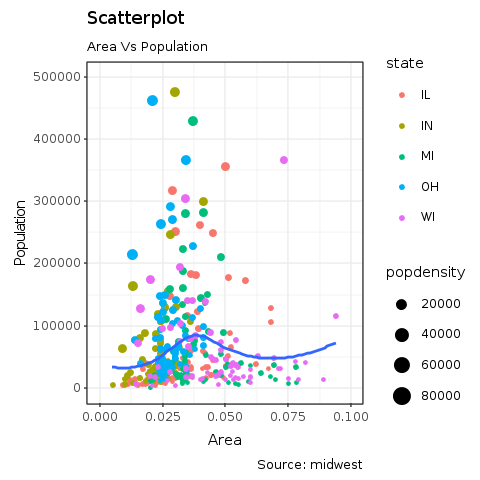
\includegraphics[width=0.7\textwidth,height=\textheight]{midwest.png}
\caption{Midwest Plot}
\end{figure}

In R, the code to generate this plot is the following

\begin{Shaded}
\begin{Highlighting}[]
\CommentTok{# install.packages("ggplot2")}
\CommentTok{# load package and data}
\KeywordTok{options}\NormalTok{(}\DataTypeTok{scipen=}\DecValTok{999}\NormalTok{)  }\CommentTok{# turn-off scientific notation like 1e+48}
\KeywordTok{library}\NormalTok{(ggplot2)}
\KeywordTok{theme_set}\NormalTok{(}\KeywordTok{theme_bw}\NormalTok{())  }\CommentTok{# pre-set the bw theme.}
\KeywordTok{data}\NormalTok{(}\StringTok{"midwest"}\NormalTok{, }\DataTypeTok{package =} \StringTok{"ggplot2"}\NormalTok{)}
\CommentTok{# midwest <- read.csv("http://goo.gl/G1K41K")  # bkup data source}

\CommentTok{# Scatterplot}
\NormalTok{gg <-}\StringTok{ }\KeywordTok{ggplot}\NormalTok{(midwest, }\KeywordTok{aes}\NormalTok{(}\DataTypeTok{x=}\NormalTok{area, }\DataTypeTok{y=}\NormalTok{poptotal)) }\OperatorTok{+}\StringTok{ }
\StringTok{      }\KeywordTok{geom_point}\NormalTok{(}\KeywordTok{aes}\NormalTok{(}\DataTypeTok{col=}\NormalTok{state, }\DataTypeTok{size=}\NormalTok{popdensity)) }\OperatorTok{+}\StringTok{ }
\StringTok{      }\KeywordTok{geom_smooth}\NormalTok{(}\DataTypeTok{method=}\StringTok{"loess"}\NormalTok{, }\DataTypeTok{se=}\NormalTok{F) }\OperatorTok{+}\StringTok{ }
\StringTok{      }\KeywordTok{xlim}\NormalTok{(}\KeywordTok{c}\NormalTok{(}\DecValTok{0}\NormalTok{, }\FloatTok{0.1}\NormalTok{)) }\OperatorTok{+}\StringTok{ }
\StringTok{      }\KeywordTok{ylim}\NormalTok{(}\KeywordTok{c}\NormalTok{(}\DecValTok{0}\NormalTok{, }\DecValTok{500000}\NormalTok{)) }\OperatorTok{+}\StringTok{ }
\StringTok{      }\KeywordTok{labs}\NormalTok{(}\DataTypeTok{subtitle=}\StringTok{"Area Vs Population"}\NormalTok{, }
           \DataTypeTok{y=}\StringTok{"Population"}\NormalTok{, }
           \DataTypeTok{x=}\StringTok{"Area"}\NormalTok{, }
           \DataTypeTok{title=}\StringTok{"Scatterplot"}\NormalTok{, }
           \DataTypeTok{caption =} \StringTok{"Source: midwest"}\NormalTok{)}

\KeywordTok{plot}\NormalTok{(gg)}
\end{Highlighting}
\end{Shaded}

Note that both codes are very similar. The Ruby code requires the use of
``R.'' before calling any functions, for instance R function
`geom\_point' becomes `R.geom\_point' in Ruby. R named parameters such
as (col = state, size = popdensity), become in Ruby (col: :state, size:
:popdensity).

One last point that needs to be observed is the call to the `aes'
function. In Ruby instead of doing `R.aes', we use `E.aes'. The
explanation of why E.aes is needed is an advanced topic in R and depends
on what is know as Non-standard Evaluation (NSE) in R. In short,
function `aes' is lazily evaluated in R, i.e., in R when calling
geom\_point(aes(col=state, size=popdensity)), function geom\_point
receives as argument something similar to a string containing
`aes(col=state, size=popdensity)', and the aes function will be
evaluated inside the geom\_point function. In Ruby, there is no Lazy
evaluation and doing R.aes would try to evaluate aes immediately. In
order to delay the evaluation of function aes we need to use E.aes. The
interested reader on NSE in R is directed to
\url{http://adv-r.had.co.nz/Computing-on-the-language.html}.

\hypertarget{an-extension-to-the-example}{%
\section{An extension to the
example}\label{an-extension-to-the-example}}

If both codes are so similar, then why would one use Ruby instead of R
and what good is galaaz after all?

Ruby is a modern OO language with numerous very useful constructs such
as classes, modules, blocks, procs, etc. The example above focus on the
coupling of both languages, and does not show the use of other Ruby
constructs. In the following example, we will show a more complex
example using other Ruby constructs. This is certainly not a very well
written and robust Ruby code, but it give the idea of how Ruby and R are
strongly coupled.

Let's imagine that we work in a corporation that has its plot themes.
So, it has defined a `CorpTheme' module. Plots in this corporation
should not have grids, numbers in labels should not use scientific
notation and the preferred color is blue.

We now define a ScatterPlot class:

And this is the final code for making the scatter plot with the midwest
data

\begin{figure}
\centering
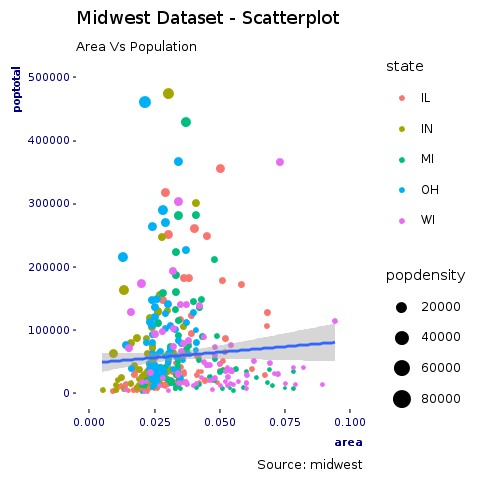
\includegraphics[width=0.7\textwidth,height=\textheight]{scatter_plot.png}
\caption{Midwest Plot with `glm' function and modified theme}
\end{figure}

\hypertarget{conclusion}{%
\section{Conclusion}\label{conclusion}}

R is a very powerful language for statistical analysis, data analytics,
machine learning, plotting and many other scientific applications with a
very large package ecosystem. However R is often considered hard to
learn and lacking modern computer languages constructs such as object
oriented classes, modules, lambdas, etc. For this reason, many
developers have started or switched from R to Python.

With Galaaz, R programmers can almost transparently migrate from R to
Ruby, since syntax is almost identical and they have fastR as the R
engine. FastR, by most benchmarks, can be orders of magnitude faster
than Gnu R. Further, by using Galaaz the R developer can start (slowly
if needed) using all of Ruby's constructs and libraries that nicely
complement R packages.

For the Ruby developer, Galaaz allows the immediate use of R functions
completely transparently. As shown in the second example above, class
ScatterPlot completely hides all the details an R calls from the Ruby
developer, furthermore Galaaz is powered by TruffleRuby that can also be
orders of magnitude faster than MRI Ruby.


\end{document}
